%
\documentclass[12pt,letterpaper]{article}
\usepackage{bbm}
\usepackage{url}
\usepackage{float}
\usepackage{fancyhdr}
%\usepackage{fancybox}
%\usepackage{amstext}
\usepackage{amsmath}
%\usepackage{rotating}
\usepackage{multicol}
\usepackage{pictexwd}
\usepackage{enumitem}
%\usepackage{booktabs}
\usepackage{graphicx}
\usepackage{booktabs,multirow}
\usepackage{siunitx}
\usepackage{subfigure}
\setlength{\parindent}{0in}
\setlength{\textwidth}{7in}
\setlength{\evensidemargin}{-0.25in}
\setlength{\oddsidemargin}{-0.25in}
\setlength{\parskip}{.5\baselineskip}
\setlength{\topmargin}{-0.65in}
\setlength{\textheight}{9in}
%               Problem and Part
\newcounter{problemnumber}
\newcounter{partnumber}
\newcommand{\Problem}{\stepcounter{problemnumber}\setcounter{partnumber}{0}\item[\makebox{\hfil\textbf{\ \theproblemnumber.}\hfil}]}
\newcommand{\Part}{\stepcounter{partnumber}\item[(\alph{partnumber})]}
\newcommand{\SubPart}{\stepcounter{problemnumber}\setcounter{partnumber}{0}}

\pagestyle{empty}

\rhead{\large\textsc{Angeline Baniqued \& Michael Wee}}
\lhead{\LARGE\textbf{CS 181 Assignment 4}}
\cfoot{}
\renewcommand{\headrulewidth}{0.3pt}
\setlength{\headsep}{40pt}
\usepackage{amssymb}

\begin{document}

\thispagestyle{fancy}\small
  \section*{Problem 1}
        \begin{enumerate}[label={(\alph*) }]
        \item 
We represent noise with parameters $p_i$ where $0 \leq p_i \leq 1$, though we assume that since this is noise, $p_i$ is more likely to be much closer to 0 than to 1. The directed graph structure is below:\ \medskip \\
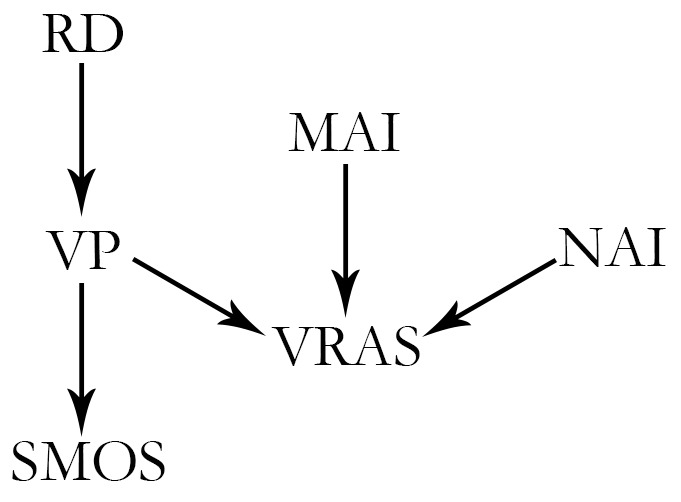
\includegraphics[width=2in]{1a.png}
\medskip\\
 The following  three variables ($p_1, p_2,$ and  $p_3$) may be easier to estimate directly and may not need noisy parameters. Depending on our certainty of our estimates, we may be able to set the first three parameters to 0, or remove them altogether from the model. Again, note that $p_i$'s are closer to 0 than to 1.\medskip \\
$P(RD = T) = 1 - p_1$ \\
$P(MAI = T) = 1 - p_2$ \\
$P(NAI = T) = 1 - p_3$ \medskip \\
Not every untrusted website leads to a virus being installed on the computer; there may be other noisy events that cause or prevent the presence of a virus.  \\

\begin{minipage}{0.3\textwidth}
        \begin{tabular}{c c c c} % centered columns (4 columns)
        \hline\hline                        %inserts double horizontal lines
         RD & P(VP$|$RD) \\ [0.5ex] 
        \hline                  % inserts single horizontal line
        T & $1-p_4$  \\ % inserting body of the table
        F & $p_5$  \\[.5ex]      
        \hline 
        \end{tabular}

        \end{minipage}\qquad \\ \medskip

Not every virus may print silly messages on screen, or some other noisy event could prevent the printing of silly messages \\

\begin{minipage}{0.3\textwidth}
        \begin{tabular}{c c c c} % centered columns (4 columns)
        \hline\hline                        %inserts double horizontal lines
         VP & P(SMOS$|$VP) \\ [0.5ex] 
        \hline                  % inserts single horizontal line
        T & 1 - $p_6$  \\ % inserting body of the table
        F & $p_7$  \\[.5ex]      
        \hline 
        \end{tabular}

        \end{minipage}\qquad \\ \medskip

This table shows that the interaction of virus reported by antivirus software is different for each combination of McAfee and Norton antivirus installed or not. When neither is installed, antivirus software cannot report a virus. When both are installed, there may be some complex interaction with them or other noise that requires detection to be a separate distribution. And when only one is installed, there is a chance that noisy events may occur, such as different efficacies of antivirus software, also requiring noisy parametrization. \\

\begin{minipage}{0.3\textwidth}
        \begin{tabular}{c c c c} % centered columns (4 columns)
        \hline\hline                        %inserts double horizontal lines
         VP & MAI & NAI & P(VRAS$|$VP, MAI, NAI) \\ [0.5ex] 
        \hline                  % inserts single horizontal line
        T & T & T & 1 - $p_8$  \\ % inserting body of the table
        T & T & F & 1 - $p_9$  \\
        T & T & T & 1 - $p_{10}$  \\
        T & F & F & 0 \\
        F & T & T & $p_{11}$  \\
        F & T & F & $p_{12}$  \\
        F & T & T & $p_{13}$  \\
        F & F & F & 0  \\  
        \hline 
        \end{tabular}

        \end{minipage}\qquad \\ \\ 
  
        \item  We could add the edge RD $\rightarrow$ VRAS. It is likely that there is a direct causal relationship between visiting an untrusted website and a detected virus by antivirus software. However, there are many other factors involved in virus detection including efficacy of antivirus programs, the fact that not all untrusted sites install viruses, or if they do, that the installation is successful. 
        \item Here is the new directed graph structure: \\
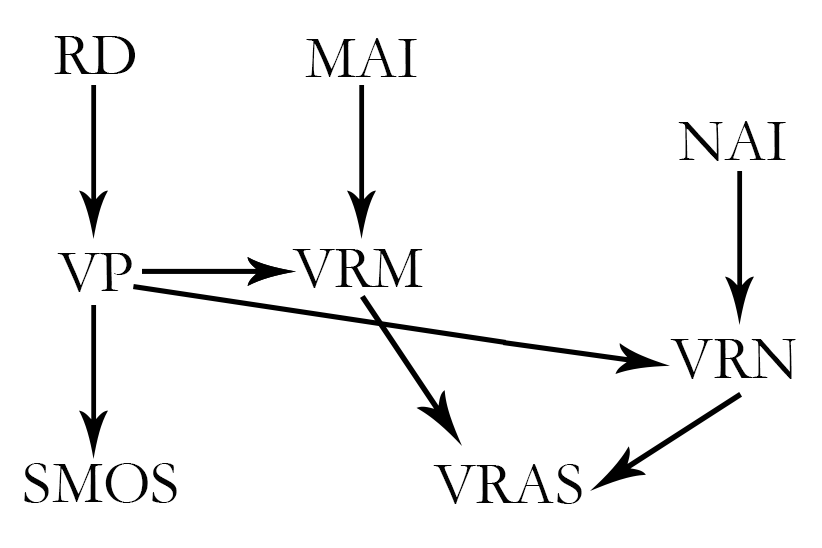
\includegraphics[width=2.5in]{1c.png}\\If McAfee antivirus is not installed, then there is a 0 probability of it reporting anything. Otherwise there may be noise we parametrize, including things such as imperfect detection by McAfee. \\

\begin{minipage}{0.3\textwidth}
        \begin{tabular}{c c c c} % centered columns (4 columns)
        \hline\hline                        %inserts double horizontal lines
         VP & MAI & P(VRM$|$VP, MAI) \\ [0.5ex] 
        \hline                  % inserts single horizontal line
        T & T & 1 - $p_{14}$  \\ % inserting body of the table
        T & F & 0  \\
        F & T & $p_{15}$  \\
        F & F & 0  \\  
        \hline 
        \end{tabular}

        \end{minipage}\qquad \\ \\ 
        

If Norton antivirus is not installed, then there is a 0 probability of it reporting anything. Otherwise there may be noise we parametrize, including things such as imperfect detection by Norton. \\

\begin{minipage}{0.3\textwidth}
        \begin{tabular}{c c c c} % centered columns (4 columns)
        \hline\hline                        %inserts double horizontal lines
         VP & NAI & P(VRM$|$VP, NAI) \\ [0.5ex] 
        \hline                  % inserts single horizontal line
        T & T & 1 - $p_{16}$  \\ % inserting body of the table
        T & F & 0  \\
        F & T & $p_{17}$  \\
        F & F & 0  \\  
        \hline 
        \end{tabular}

        \end{minipage}\qquad \\ \\ 
        
The following relationship has the same truth table as the OR relation. If either McAfee or Norton reports a virus, then an antivirus software has detected a virus by definition. There is no need to account for noise here. \\

\begin{minipage}{0.3\textwidth}
        \begin{tabular}{c c c c} % centered columns (4 columns)
        \hline\hline                        %inserts double horizontal lines
         VRM & VRN & P(VRAS$|$VRM, VRN) \\ [0.5ex] 
        \hline                  % inserts single horizontal line
        T & T & 1  \\ % inserting body of the table
        T & F & 1  \\
        F & T & 1  \\
        F & F & 0  \\  
        \hline 
        \end{tabular}

        \end{minipage}\qquad \\ \\      
        
 \item

Adding VRM and VRN hinders the modeling process. It does not matter to us whether individual antivirus programs detect viruses (we are not testing efficacy of antivirus programs) but whether a virus is detected by an antivirus program. VRM and VRN provide no new useful information as they feed directly into VRAS. In conclusion, they hinder the modeling process by introducing new variables, more conditional probabilities, and more variables that are not that straightforward to sum and marginalize over. \\
\end{enumerate}
\section*{Problem 2}
\begin{enumerate}[label={(\alph*) }]
        \item
 
For graph (a), none of the variables are conditionally independent of A given B. This is because information still flows to A from G through E and C to A, so all of these are still conditionally dependent given B. Information flows from F to A through F and C to A so all of these are conditionally dependent. I is still conditionally dependent because information flows through H since it exhibits a tail to tail relationship with the path through I and F. Information flows from D to G, since G is tail-to-tail to the path through D and E and from G to A. \\

For graph (b), variables C and F are conditionally independent of A given J. Variable G exhibits a head to head relationship with the path through A and D but we know its descendant J, so it does not block any path that flows to G through D. All paths to A from C and F must go through I, but I is head-to-head with the path through F and E, and none of its children are known, so it blocks C and F from the path to A so C and F are conditionally independent of A given J.  \\  

\item
For graph (a), the joint probability factorization is as follows: \medskip \\
$P(A, B, C, D, E, F, G, H, I) = \\ P(A|B, C)P(B|D)P(C|E,F)P(D|G)P(E|G)P(F|H)P(G)P(H)P(I|H,G)$ \\

For graph (b), the joint probability factorization is as follows:  \medskip \\
$P(A, B, C, D, E, F, G, H, I,J) = \\ P(A)P(B)P(C)P(D|B)P(E|B)P(F|C)P(G|A,D)P(H|D,E)P(I|E,F)P(J|G)$ \\

\newpage


        \item Factor graph representation of $(a):$ \\
        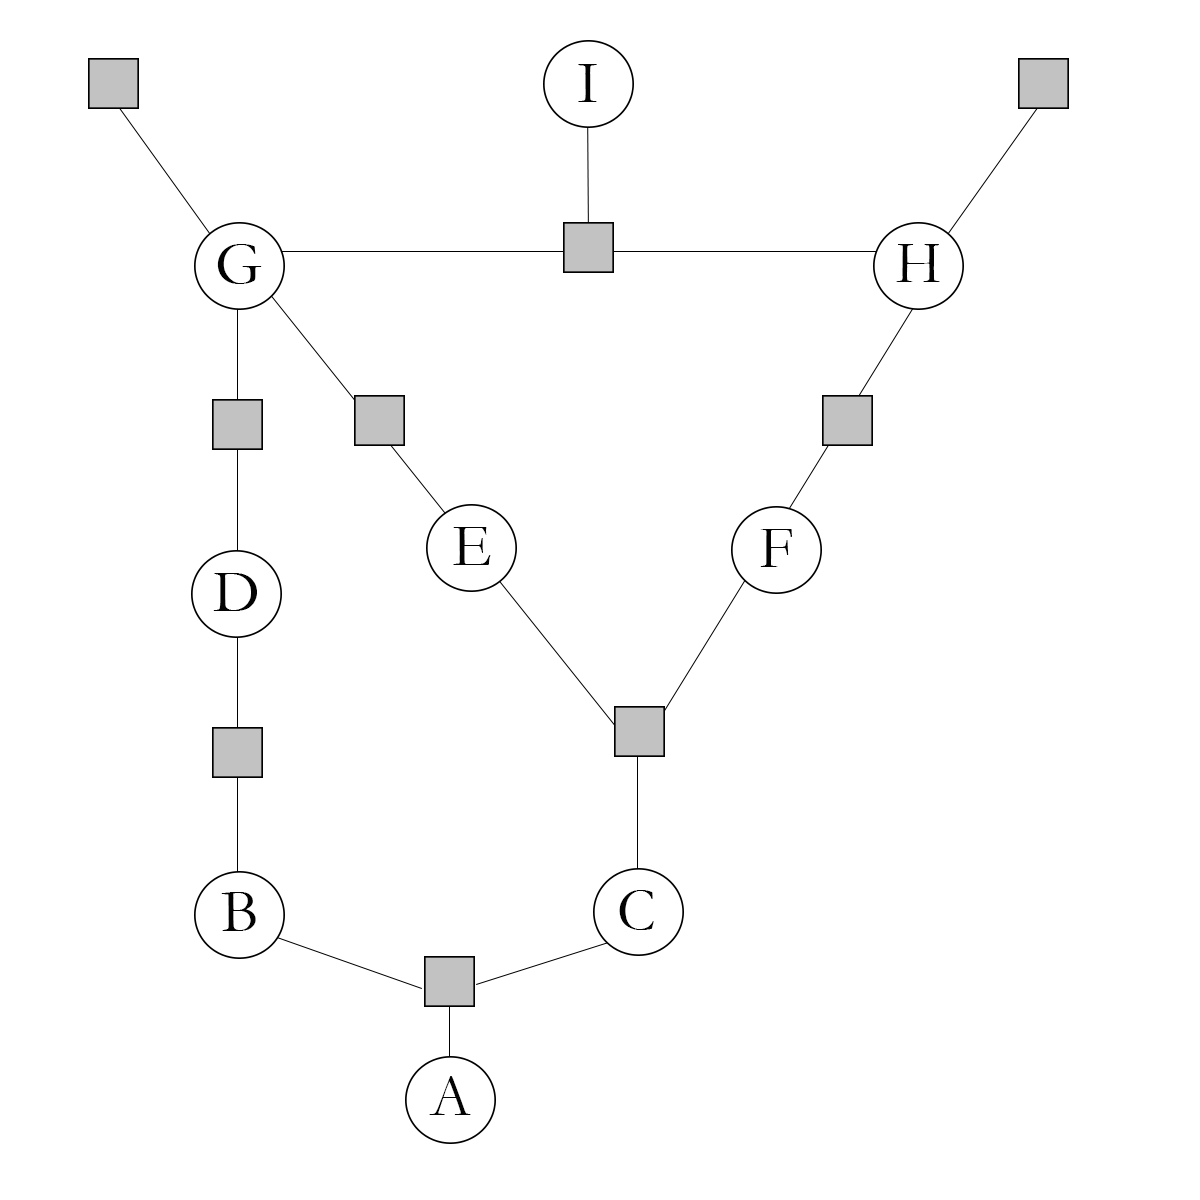
\includegraphics[width=4in]{2c_a.png}\\
        Factor graph representation of $(b):$ \\
        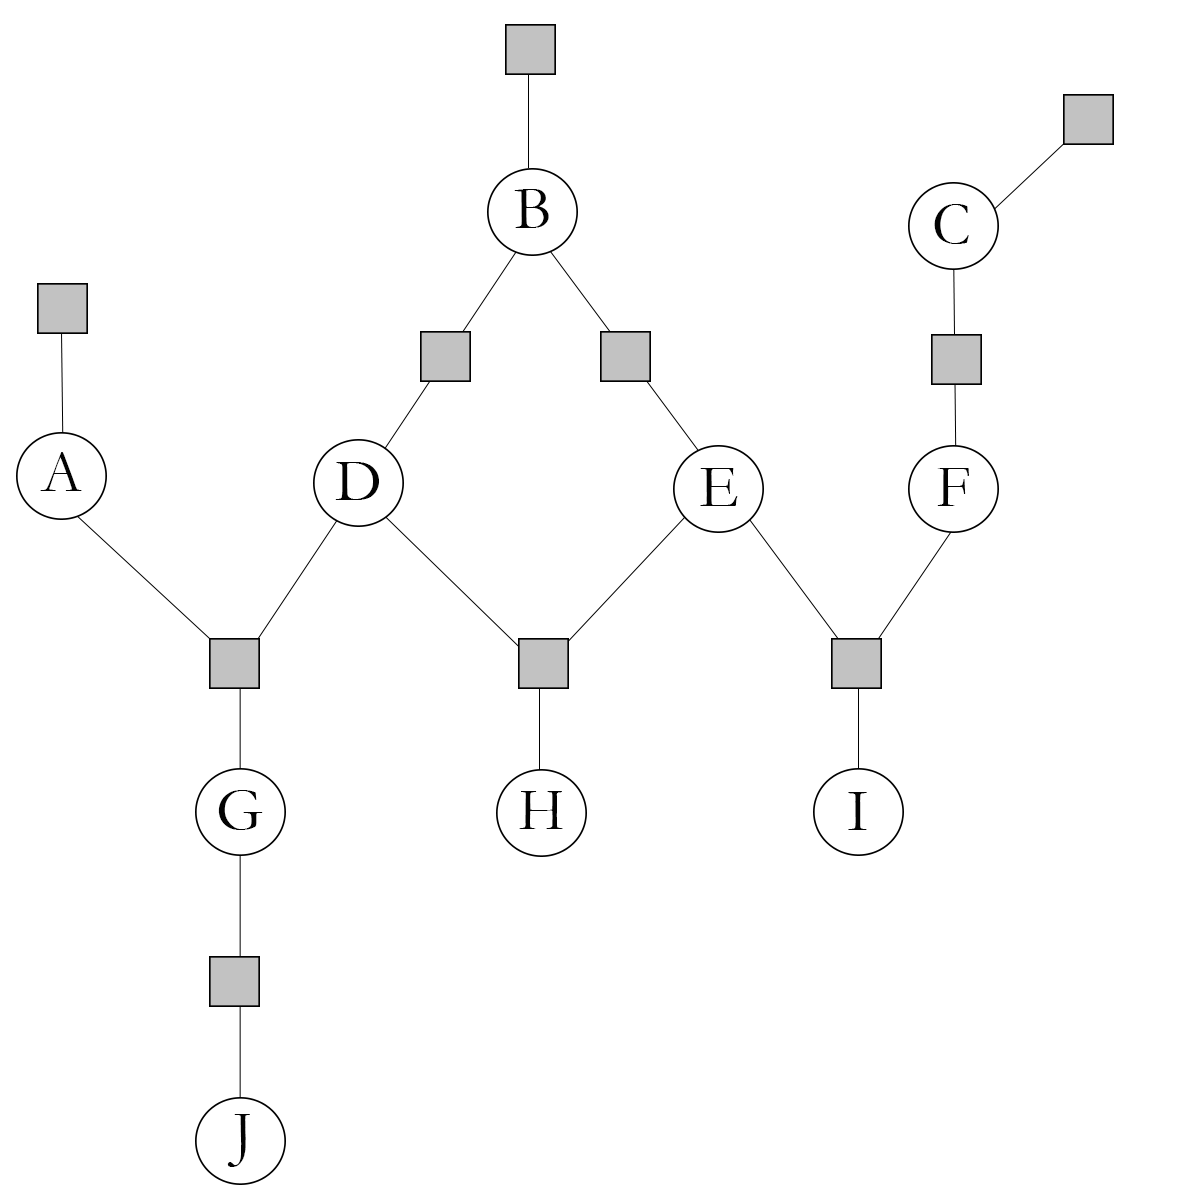
\includegraphics[width=4in]{2c_b.png} \\
        \newpage
        \item Undirected graphical model representation of $(a):$\\
        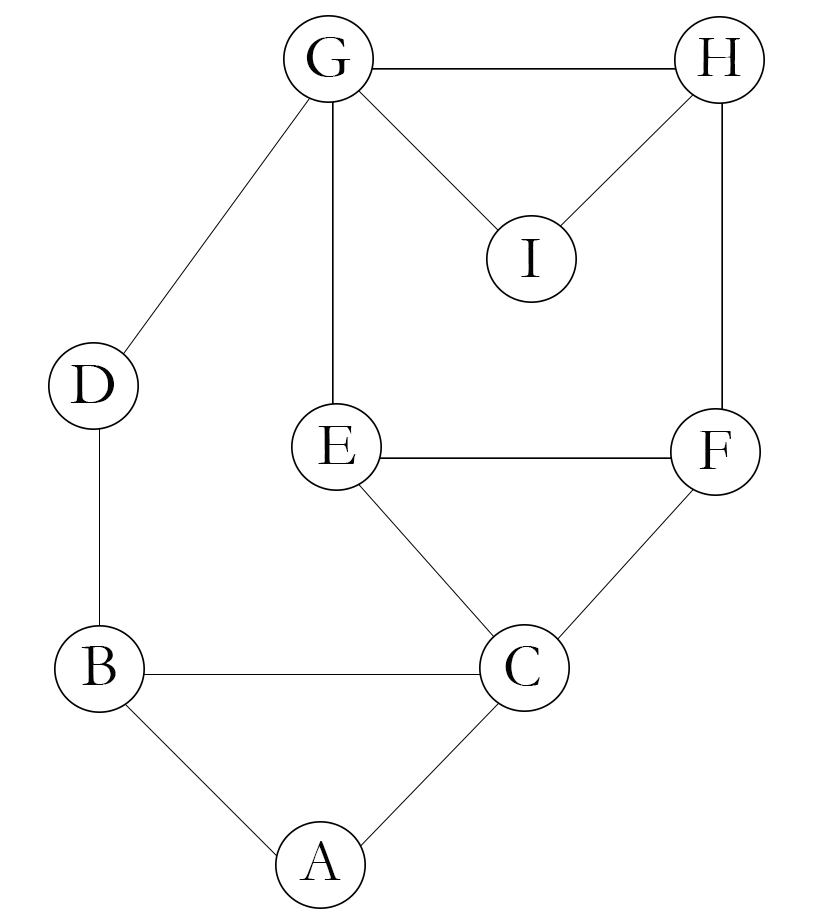
\includegraphics[width=2.75in]{2d_a.png}\medskip \\
        Undirected graphical model representation of $(b):$\\
        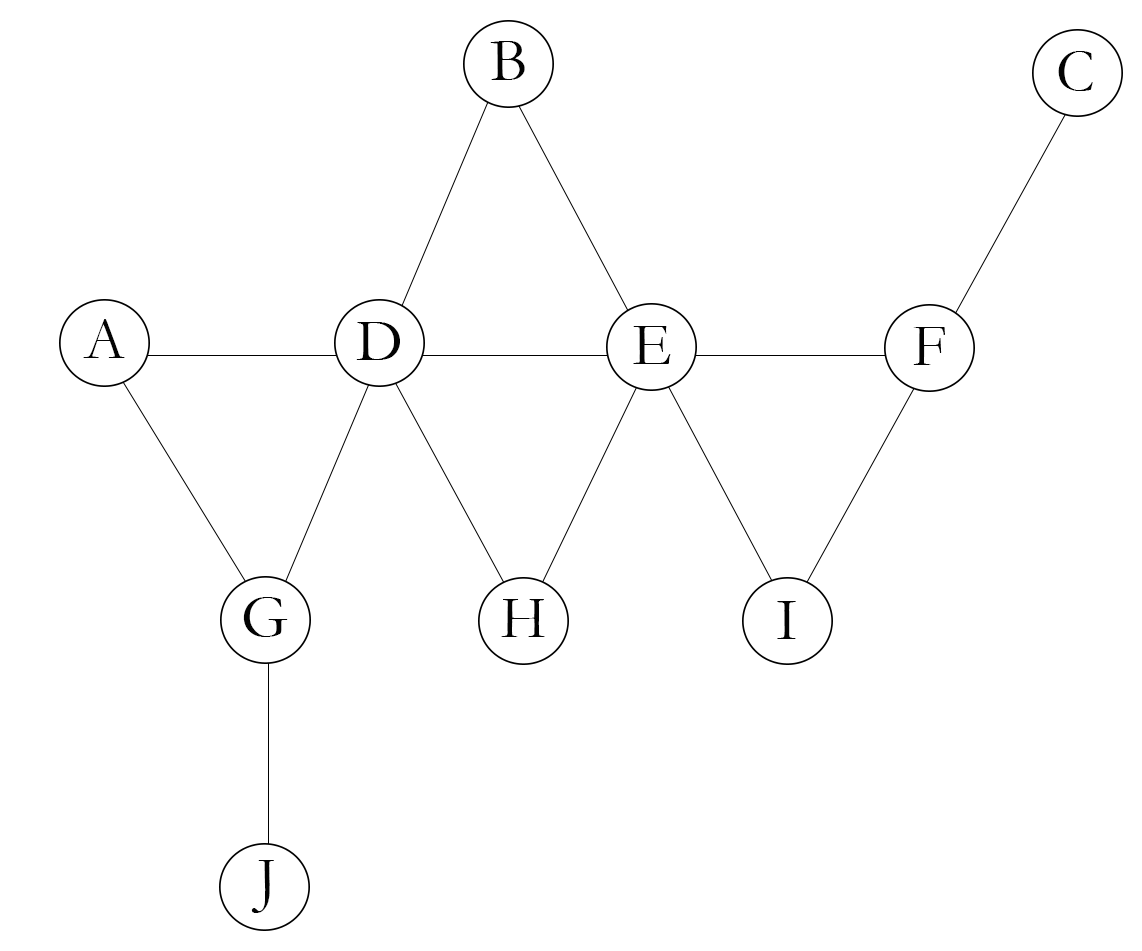
\includegraphics[width=4in]{2d_b.png}
        \end{enumerate}
  \section*{Problem 3}
        \begin{enumerate}[label={(\alph*) }]
                \item The density function of the mixture of Gaussians distributions is below: \\
                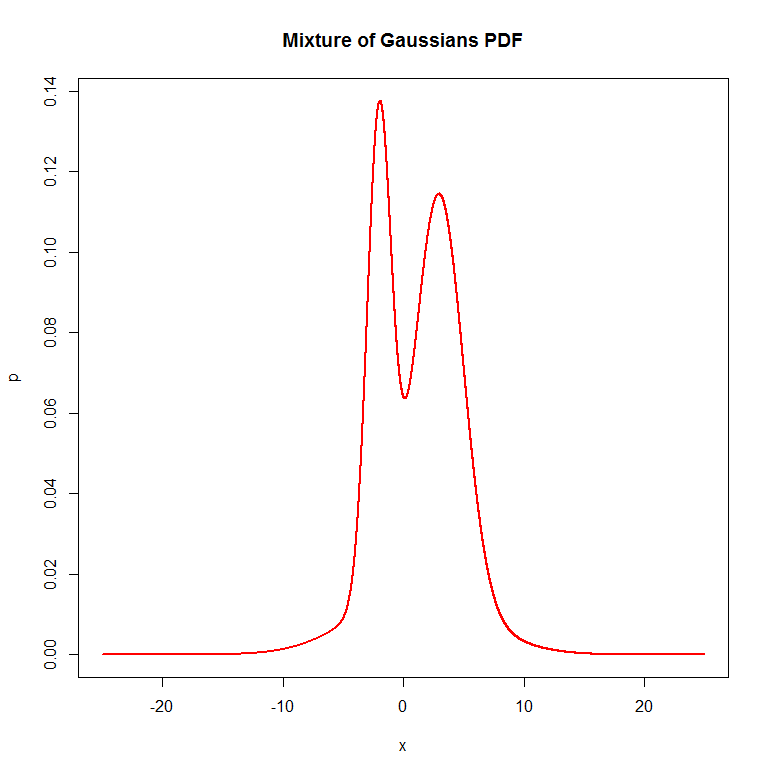
\includegraphics[width=3.5in]{3a_pdf.png}
                \item A way to generate data from this distribution is to start by generating 500 samples from a standard uniform distribution. After which, if the sample is $<2$, then we'll draw from a $\mathcal{N}(1,25)$ distribution. If the sample were $>=.2$ and $<.5$, then we'll draw from a $\mathcal{N}(-2,1)$ distribution. Lastly, if the same were $>=.5$ and $<1$, then we'll draw from a $\mathcal{N}(3,4)$. This procedure produces the following plot: \\
                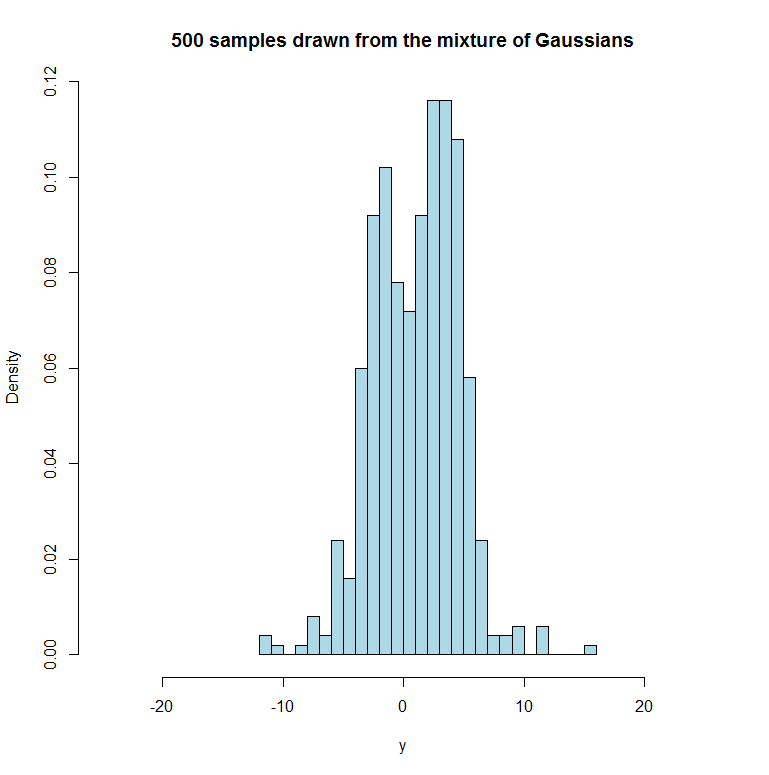
\includegraphics[width=3.5in]{3b_hist.png}
                \item The upper bounding function we chose is the $2.75* \mathcal{N}(1.5,30)$ distribution, where $c=0.75$ and $q(x)\sim\mathcal{N}(1.5,30) $. We started with other values of $c$, but we wanted an upper bound that was somewhat close to the actual distribution so $2.75$ seemed like a reasonable choice.
In addition, we chose the $\mathcal{N}(1.5,30)$ because we wanted the mean to be close to the peak of the density function and we chose 30 because wanted the variance to be greater than the variances of the individual Gaussians to ensure that our upper bound is always above the mixture of Gaussians distribution. To verify that it is always an upper bound, we set the two $PDF$s equal to each other, and indeed, they never intersect. Plotted together, the two functions look like this: \\
        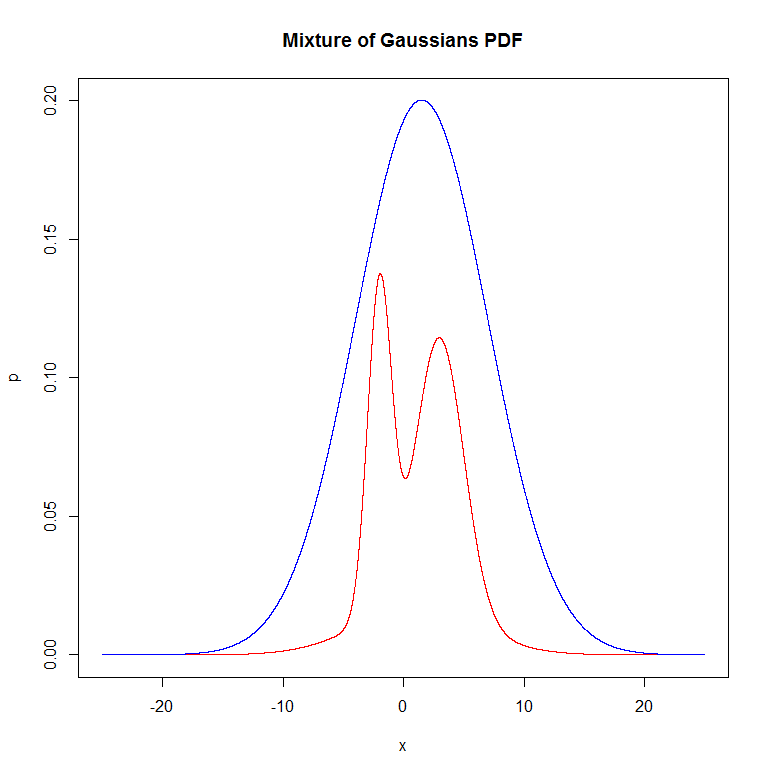
\includegraphics[width=3.5in]{3c_upper_lower.png} \\
        
        After drawing 500 samples from the upper bound and accepting samples that were below $\pi(x)$, we get the following histogram. For ease of comparison, we also plotted $\pi(x)$ below: \\
        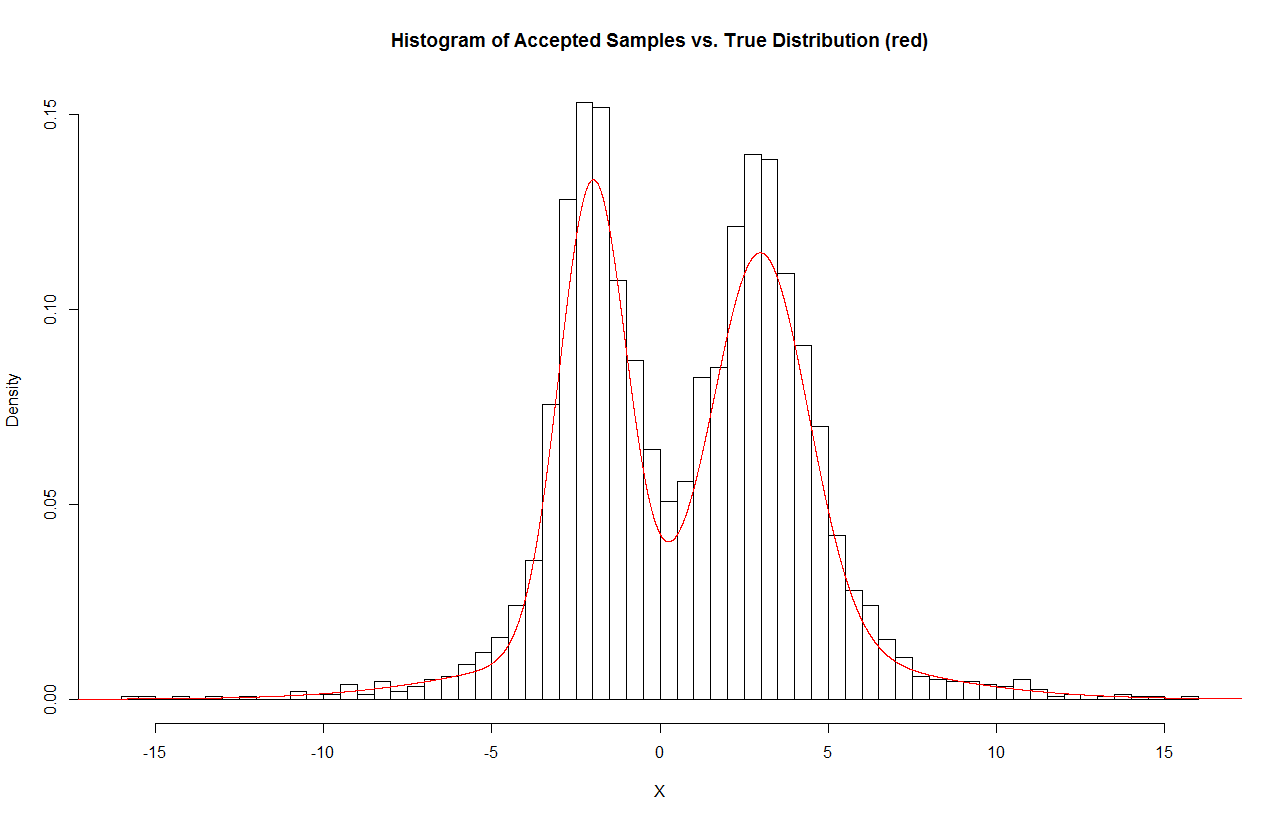
\includegraphics[width=3.5in]{3c_accepted_true.png}\\
        
        Lastly, the following visualization also shows you the rejection vs. the acceptance region from running the rejection sampler. \\
        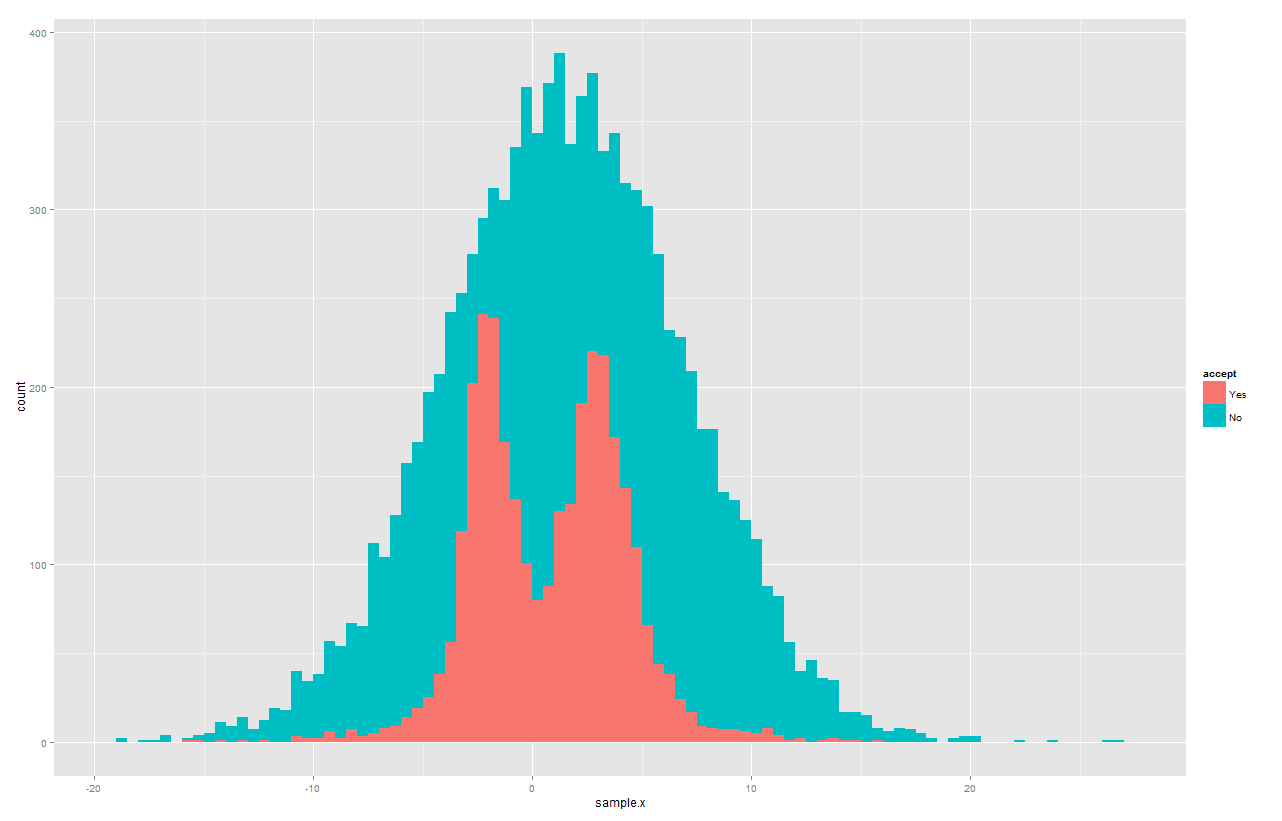
\includegraphics[width=3.5in]{3c_accept_reject_region.png}\\
        
        With our chosen upper bound, we got 866 rejections before getting 500 acceptances. 
        
      \item Here's a list of variances and acceptance rates that we tried:\\
       \begin{tabular}{c c} % centered columns (4 columns)
        \hline\hline                        %inserts double horizontal lines
         Variance & Acceptance Rate (acceptances/samples) \\ [0.5ex] 
        \hline                  % inserts single horizontal line
        0.1 & 0.95   \\
        0.3 & 0.93   \\  
        0.5 & 0.91 \\
        1.0 & 0.86 \\
        2.0 & 0.82 \\
        4.0 & 0.74 \\
        10.0 & 0.69 \\
        \hline 
        \end{tabular}\medskip \\
        
        As can be observed from the table, if the variance is too small, then the acceptance rate will be high. Because you're proposing consecutive samples that will be  very close to one another and this will lead to slow convergence. \medskip \\
 On the other hand, if the variance is too large, the acceptance rate will be relatively low. Because the proposals will tend to land in the more extreme regions and will tend to be far apart, causing the convergence to be really slow given that you remain at the same point for a number of iterations.

        The histograms that support these results for the different variances are below: \\
        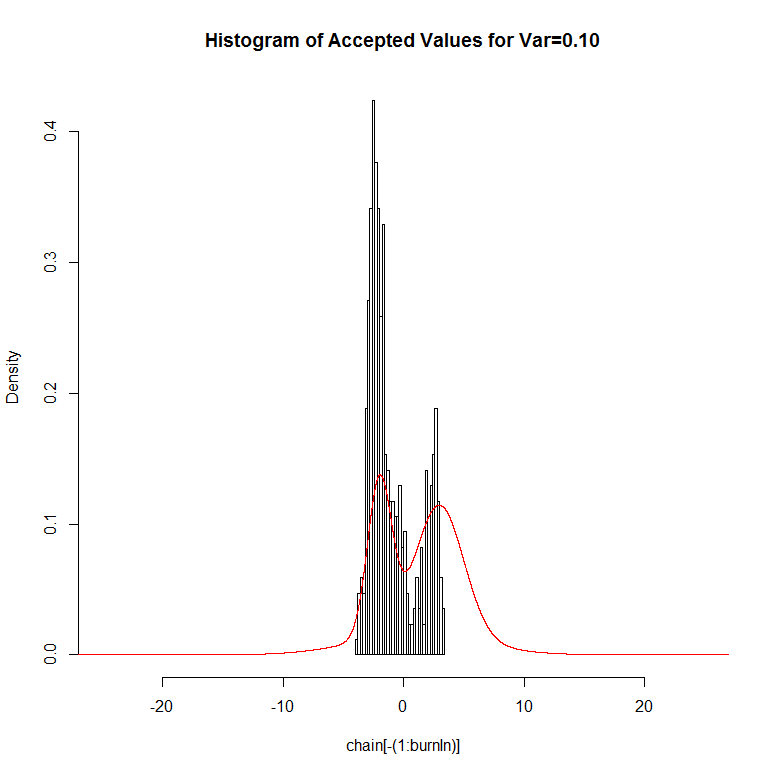
\includegraphics[width=3in]{3d_p1.png} 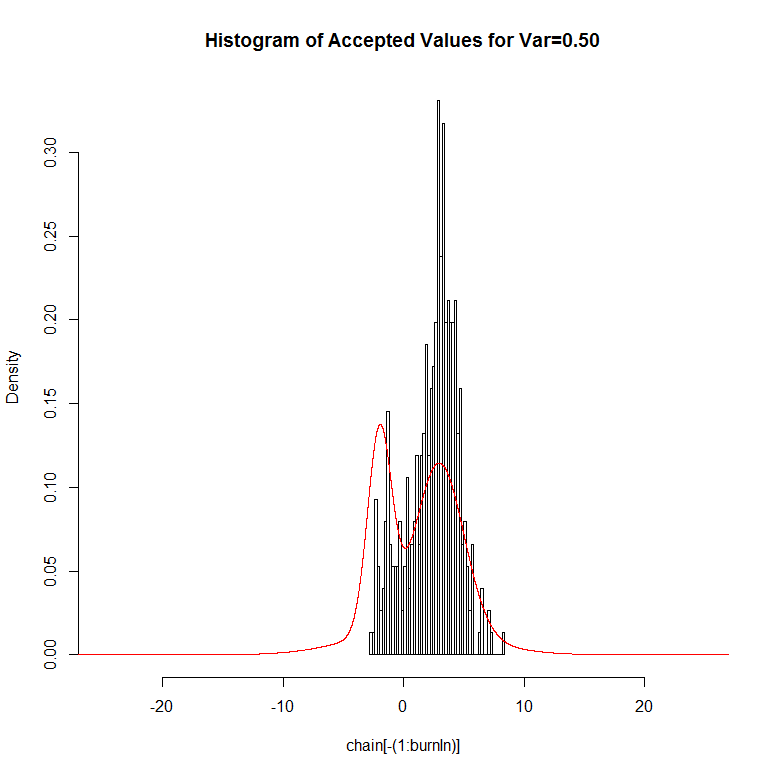
\includegraphics[width=3in]{3d_p5.png} \\
        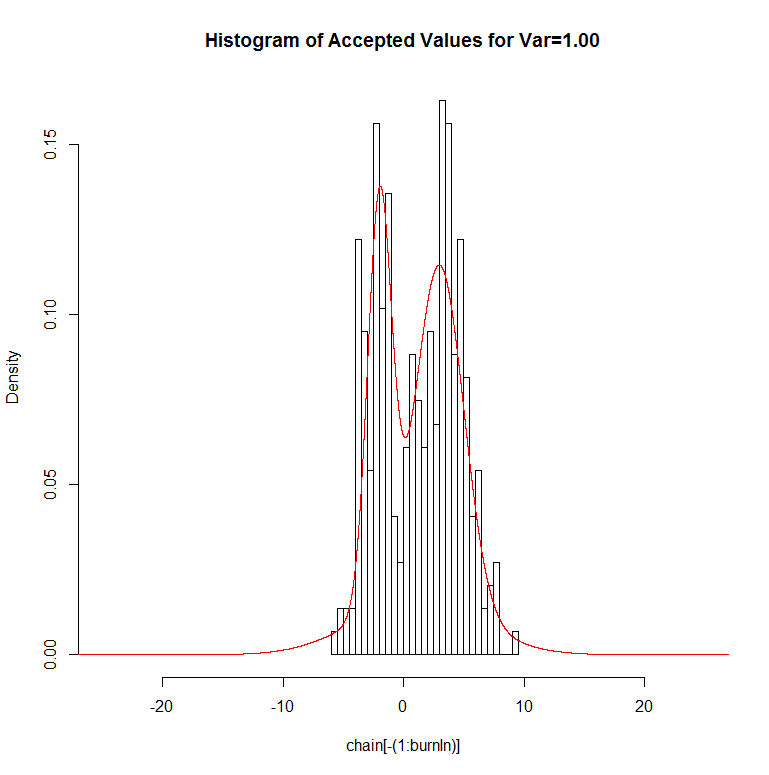
\includegraphics[width=3in]{3d_1.png} 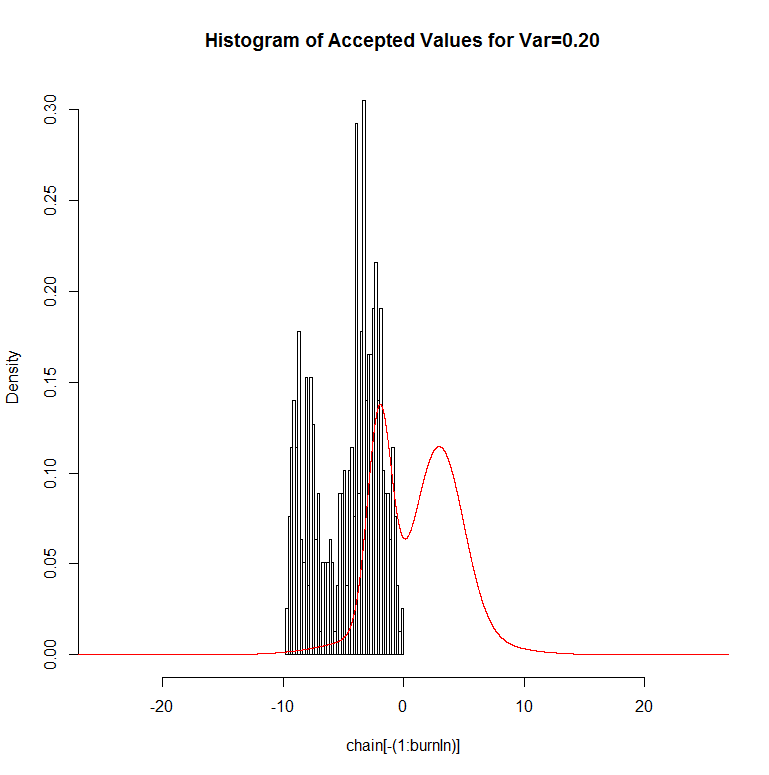
\includegraphics[width=3in]{3d_p2.png} \\
        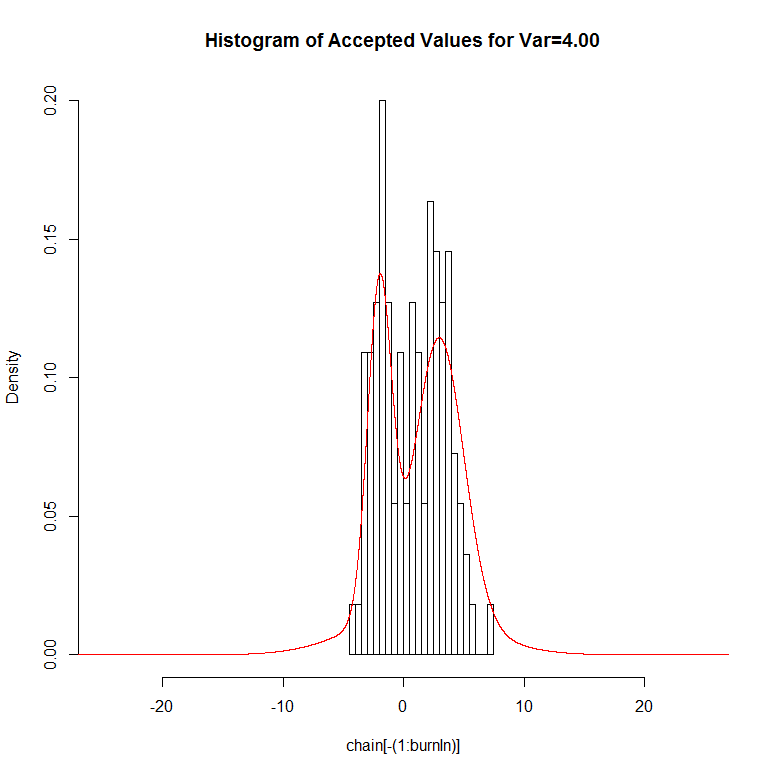
\includegraphics[width=3in]{3d_4.png} 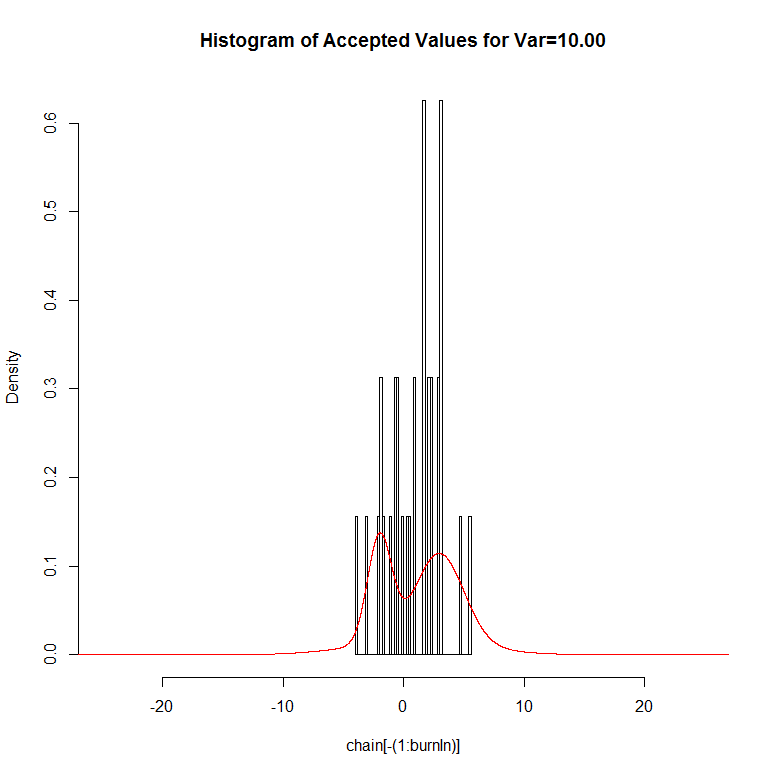
\includegraphics[width=3in]{3d_10.png} \\
   
   \end{enumerate}
\end{document}
